% Lecture 13, Fig. 1: the motion maps the reference body M to the instantaneous body M_t.
\documentclass[tikz,border=6pt]{standalone}
\usepackage{mathpazo}
\usepackage{bm}
\begin{document}
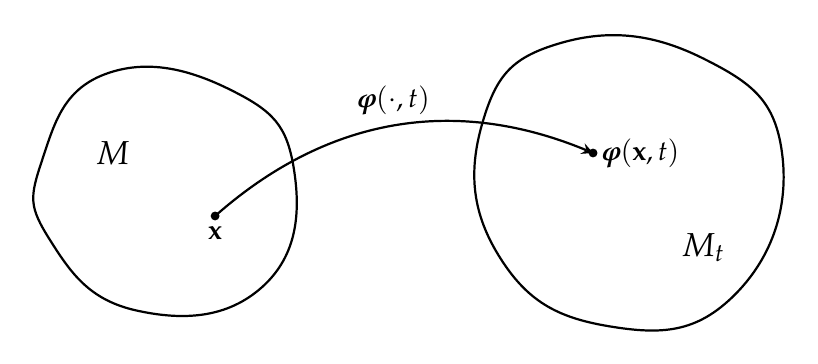
\begin{tikzpicture}[line width=0.8pt]
  % reference body M
  \draw plot[smooth cycle, tension=0.8] coordinates
    {(-4.4,0.4) (-3.6,1.5) (-2.0,1.3) (-1.2,0.3) (-1.6,-1.2) (-3.2,-1.5) (-4.3,-0.6)};
  \node at (-3.5,0.5) {\large $M$};
  \fill (-2.2,-0.3) circle (1.6pt);
  \node[below] at (-2.2,-0.3) {$\mathbf{x}$};
  % instantaneous body M_t
  \draw plot[smooth cycle, tension=0.8] coordinates
    {(1.2,0.9) (2.2,1.9) (4.0,1.7) (5.0,0.5) (4.4,-1.3) (2.8,-1.7) (1.4,-0.8)};
  \node at (4.0,-0.7) {\large $M_{t}$};
  \fill (2.6,0.5) circle (1.6pt);
  \node[right] at (2.6,0.5) {$\bm{\varphi}(\mathbf{x},t)$};
  % the motion
  \draw[->,>=stealth] (-2.2,-0.3) to[bend left=32] node[above,midway] {$\bm{\varphi}(\cdot,t)$} (2.6,0.5);
\end{tikzpicture}
\end{document}
